\chapter{Modelo del levitador ECP-730}\label{chap:modelo}

El capítulo~\ref{chap:introduccion} presentó el problema y el capítulo~\ref{chap:fundamentos} reunió las herramientas con las que se aborda. Este capítulo responde a la pregunta que sigue: qué planta se va a controlar y qué límites impone. Se construye el modelo término a término, desde la fuerza electromagnética hasta la fricción y la zona muerta del actuador, se linealiza alrededor de un equilibrio para obtener el modelo con el que se diseña el controlador, se observa cómo se comporta la planta sin control y, por último, se examina qué puede y qué no puede hacer el actuador. Esto último fija el intervalo de posiciones en el que tiene sentido trabajar.

\section{Ecuación de movimiento}\label{sec:ec_movimiento}

La dinámica del imán en el sistema de levitación magnética ECP~\cite{730}, con la bobina superior activada, obedece la segunda ley de Newton. Se trata de la ecuación de movimiento~\eqref{eq:intro_modelo} de la introducción, que aquí se escribe con la fuerza electromagnética sin especificar,
\begin{equation}
m\ddot{x} = f_{\text{fld}}(u,x) - f_{\text{fr}} - mg .
\label{eq:mec}
\end{equation}
En la ecuación de movimiento~\eqref{eq:mec}, $m$ es la masa del imán, en kilogramos, y $\ddot{x}$ su aceleración, en $\text{cm}/\text{s}^2$. La fuerza electromagnética $f_{\text{fld}}$ que ejerce la bobina depende del voltaje aplicado $u$ y de la posición $x$, y se opone al peso $mg$ del imán. La fuerza de fricción $f_{\text{fr}}$ proviene del contacto del imán con su varilla guía. Todas las fuerzas se expresan en $\text{kg}\cdot\text{cm}/\text{s}^2$, en coherencia con los parámetros de la tabla~\ref{tab:parametros}.

La posición $x$ del imán se mide sobre el eje vertical y crece hacia la bobina superior; con el modelo de fuerza que se adopta más adelante, la distancia entre el imán y esa bobina es $a-x$. Por ello, los valores negativos de $x$ que se emplean en este trabajo corresponden a posiciones más alejadas de la bobina, que requieren un voltaje de equilibrio mayor. La figura~\ref{fig:dispositivo} muestra el esquema del dispositivo y las fuerzas que actúan sobre el imán.

\begin{figure}[ht]
    \centering
    % Esquema del ECP-730 en configuración atractiva (notación de la tesis).
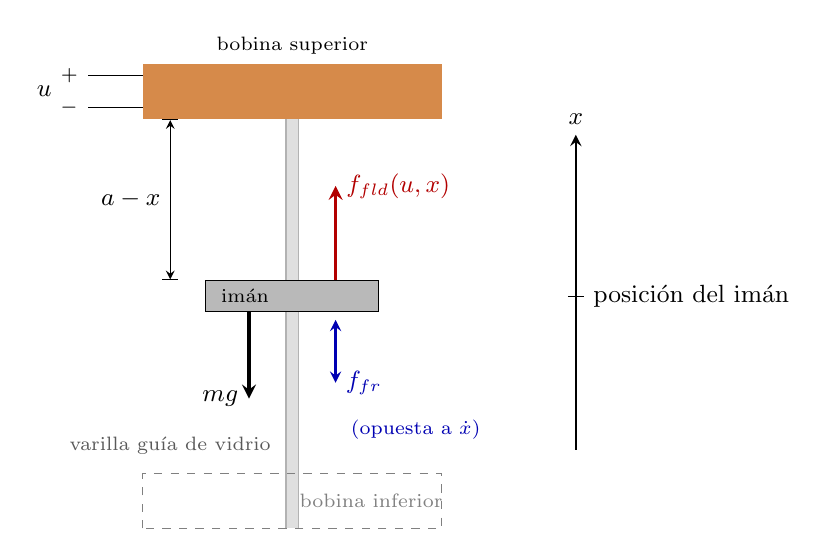
\begin{tikzpicture}[>=stealth, font=\small]
  \definecolor{cobre}{RGB}{214,138,74}
  % varilla guía
  \fill[gray!25] (-0.08,-3.6) rectangle (0.08,2.15);
  \draw[gray!60] (-0.08,-3.6) -- (-0.08,2.15) (0.08,-3.6) -- (0.08,2.15);
  \node[gray!70!black, anchor=east, font=\scriptsize] at (-0.15,-2.55) {varilla guía de vidrio};
  % bobina superior (activa)
  \fill[cobre] (-1.9,1.6) rectangle (1.9,2.3);
  \node[above, font=\scriptsize] at (0,2.3) {bobina superior};
  \draw (-1.9,2.15) -- (-2.6,2.15) node[left, font=\scriptsize] {$+$};
  \draw (-1.9,1.75) -- (-2.6,1.75) node[left, font=\scriptsize] {$-$};
  \node at (-3.15,1.95) {$u$};
  % bobina inferior (inactiva en esta configuración)
  \draw[dashed, gray] (-1.9,-3.6) rectangle (1.9,-2.9);
  \node[gray, font=\scriptsize] at (1.0,-3.25) {bobina inferior};
  % imán levitante
  \fill[gray!55] (-1.1,-0.85) rectangle (1.1,-0.45);
  \draw (-1.1,-0.85) rectangle (1.1,-0.45);
  \node[font=\scriptsize] at (-0.6,-0.65) {imán};
  % fuerzas
  \draw[->, very thick, red!70!black] (0.55,-0.45) -- (0.55,0.75) node[right] {$f_{\text{fld}}(u,x)$};
  \draw[->, very thick] (-0.55,-0.85) -- (-0.55,-1.95) node[left] {$mg$};
  \draw[<->, thick, blue!70!black] (0.55,-0.95) -- (0.55,-1.75) node[right] {$f_{\text{fr}}$};
  \node[blue!70!black, font=\scriptsize, anchor=north west] at (0.62,-2.1) {(opuesta a $\dot x$)};
  % distancia a la bobina
  \draw[|<->|, thin] (-1.55,-0.45) -- (-1.55,1.6) node[midway, left] {$a-x$};
  % eje x
  \draw[->, thick] (3.6,-2.6) -- (3.6,1.4) node[above] {$x$};
  \draw (3.5,-0.65) -- (3.7,-0.65) node[right] {posición del imán};
\end{tikzpicture}

    \caption[Esquema del ECP-730 en configuración atractiva]{Esquema del sistema de levitación ECP-730 en configuración atractiva. La bobina superior atrae al imán, que se desliza sobre una varilla guía; el contacto entre ambos produce la fricción $f_{\text{fr}}$. La bobina inferior solo se emplea en la configuración repulsiva.}
    \label{fig:dispositivo}
\end{figure}

\section{\texorpdfstring{Fuerza electromagnética $f_{\text{fld}}$}{Fuerza electromagnética}}\label{sec:fuerza}

La literatura documenta varias formas no lineales para la fuerza electromagnética, que dependen de cómo varía la inductancia de la bobina con la posición del objeto levitante. De acuerdo con Al-Muthair y Zribi~\cite{al}, la fuerza sobre una bola ferromagnética levitada se aproxima por
\begin{equation}
f_{\text{fld}} = C\left(\dfrac{i}{x}\right)^2 .
\label{eq:fld_al}
\end{equation}
En la aproximación de Al-Muthair~\eqref{eq:fld_al}, la fuerza crece con el cuadrado de la intensidad de corriente $i$ y decrece con el cuadrado de la posición $x$ de la bola. La constante $C$ de la fuerza magnética reúne las propiedades del electroimán.

Charara et al.~\cite{charara} calculan la fuerza electromagnética dentro de un cojinete magnético como
\begin{equation}
f_{\text{fld}} = K\,\frac{\operatorname{sign}(i)\,i^{2}}{e^{2}},
\qquad
K = 0{,}25 \cos\!\left(\frac{\pi}{8}\right)\!\mu\, n^{2} S .
\label{eq:fld_charara}
\end{equation}
En el modelo del cojinete~\eqref{eq:fld_charara}, la fuerza conserva el signo de la corriente $i$ y decrece con el cuadrado del entrehierro $e$. La constante $K$ depende del área $S$ de la cara del polo, de la permeabilidad magnética del vacío $\mu$ y del número $n$ de vueltas del embobinado.

El Hajjaji y Ouladsine~\cite{el} determinaron experimentalmente que la fuerza electromagnética sobre una esfera metálica tiene la forma
\begin{equation}
f_{\text{fld}} = \dfrac{i^{2}}{b_0 + b_1x + b_2x^3 + b_3x^4} .
\label{eq:fld_hajjaji}
\end{equation}
Los coeficientes del ajuste experimental~\eqref{eq:fld_hajjaji} son $b_0=0{,}0304$, $b_1=0{,}7159$, $b_2=-0{,}9165$ y $b_3=1{,}1994$.

Zhao et al.~\cite{zhao} calculan la fuerza del electroimán que hace levitar una bola metálica como
\begin{equation}
f_{\text{fld}} = \frac{L_0 x_0 i^2}{2x^2} .
\label{eq:fld_zhao}
\end{equation}
La fuerza del modelo de Zhao~\eqref{eq:fld_zhao} crece con el cuadrado de la corriente $i$ del embobinado y decrece con el cuadrado de la posición $x$ de la bola. Su escala la fija la inductancia $L_0$ del sistema en el punto de equilibrio $x_0$.

Zhang y Suyama~\cite{feifei} determinan, para un sistema similar, la fuerza electromagnética
\begin{equation}
f_{\text{fld}} = \frac{K i^2}{(H - x)^2} .
\label{eq:fld_zhang}
\end{equation}
La fuerza del modelo de Zhang~\eqref{eq:fld_zhang} también crece con el cuadrado de la intensidad de la corriente $i$, y su denominador depende de la posición $x$ del objeto. Las constantes $K$ y $H$ son parámetros del sistema.

Cada uno de estos modelos está condicionado por la configuración del sistema y por la metodología, analítica o experimental, con que se obtuvo. Por ello, en este trabajo se adopta el modelo del levitador ECP-730 que da el fabricante en su hoja de especificaciones~\cite{parks}, validado experimentalmente por Hernández Alcántara et al.~\cite{alcantara},
\begin{equation}
f_{\text{fld}} = \frac{u}{b(a-x)^4} .
\label{eq:fld}
\end{equation}
La fuerza del fabricante~\eqref{eq:fld} es proporcional al voltaje $u$ aplicado en las terminales del embobinado del electroimán y decrece con la cuarta potencia de la distancia $a-x$ entre el imán, en la posición $x$, y la bobina. Los parámetros $a$ y $b$ son propios del dispositivo y se reúnen en la tabla~\ref{tab:parametros}.

Con la fuerza del fabricante, el imán en reposo y sin fricción permanece en equilibrio en la posición $x$ cuando el voltaje es
\begin{equation}
u_e(x) = mg\,b\,(a-x)^4 .
\label{eq:ue}
\end{equation}
El voltaje de equilibrio~\eqref{eq:ue} es el que hace que la fuerza electromagnética compense el peso. Crece con la cuarta potencia de la distancia a la bobina, y la zona muerta del actuador, que se describe en la sección~\ref{sec:zm_modelo}, se centra en él.

\subsection{Justificación de primeros principios}\label{sec:fuerza_primeros_principios}

Los modelos~\eqref{eq:fld_al}--\eqref{eq:fld_zhang} comparten la forma $i^2/\text{entrehierro}^2$, propia de un electroimán cuya armadura ferromagnética está cerca de la cara del polo. La energía almacenada en un circuito magnético con un entrehierro simple, de inductancia $L(x)=\mu_0 N^2 S/[2(a-x)]$, con $N$ vueltas y área de polo $S$, da la fuerza de reluctancia
\begin{equation}
f_{\text{rel}} = \frac{1}{2}\,i^2\,\frac{dL}{dx} = \frac{\mu_0 N^2 S\, i^2}{4\,(a-x)^2} ,
\label{eq:fld_reluctancia}
\end{equation}
que reproduce la forma de los modelos de la literatura citados: cuadrática en la corriente $i$ y decreciente con el cuadrado del entrehierro.

El ECP-730, en su configuración atractiva, no acerca una armadura a la cara del polo: el imán permanente se mantiene a una distancia $a$ del orden del tamaño de la propia bobina, no mucho menor que él. En ese régimen conviene aproximar tanto la bobina como el imán por dipolos magnéticos puntuales sobre el mismo eje. El campo axial, lejos de un dipolo de momento $m_{\text{bob}}$, es
\begin{equation}
B(z) = \frac{\mu_0}{4\pi}\,\frac{2\,m_{\text{bob}}}{z^3} ,
\label{eq:campo_dipolo}
\end{equation}
con $z$ la distancia sobre el eje. La energía de interacción con un imán de momento $m_{\text{im}}$ alineado es $U(z)=-m_{\text{im}}B(z)=-\mu_0 m_{\text{im}} m_{\text{bob}}/(2\pi z^3)$, menor cuanto más cerca está el imán de la bobina, como corresponde a una interacción atractiva. La componente de la fuerza sobre el eje $z$ es la pendiente de esa energía, con signo cambiado,
\begin{equation}
f_z(z) = -\frac{dU}{dz} = -\frac{3\,\mu_0\, m_{\text{im}}\, m_{\text{bob}}}{2\pi\, z^4} .
\label{eq:fuerza_dipolo}
\end{equation}
El signo negativo de~\eqref{eq:fuerza_dipolo} es correcto y esperado: $f_z$ apunta hacia $z$ decreciente, es decir, hacia la bobina, que es justo el sentido de la atracción. Para expresar la fuerza en términos de la posición $x$ del imán hace falta pasar de la variable $z$, que mide la separación, a la variable $x$ de la figura~\ref{fig:dispositivo}, que crece hacia la bobina; la relación es $z=a-x$, de modo que $dz/dx=-1$ y la regla de la cadena invierte el signo,
\begin{equation}
f_{\text{dip}}(x) = -\frac{d}{dx}\big[U(a-x)\big] = f_z(a-x)\cdot\frac{dz}{dx} = \frac{3\,\mu_0\, m_{\text{im}}\, m_{\text{bob}}}{2\pi\, (a-x)^4} .
\label{eq:fuerza_dipolo_x}
\end{equation}
La fuerza~\eqref{eq:fuerza_dipolo_x}, ahora positiva, empuja al imán en el sentido de $x$ creciente, hacia la bobina, como corresponde a la fuerza de atracción que entra en la ecuación de movimiento~\eqref{eq:mec}. A diferencia de la fuerza de reluctancia~\eqref{eq:fld_reluctancia}, decrece con la cuarta potencia de la separación, como el modelo del fabricante. Falta relacionar el momento de la bobina con el voltaje aplicado. Como la bobina es resistiva y su constante de tiempo eléctrica es mucho menor que la mecánica, la corriente sigue al voltaje casi instantáneamente, $i=u/R$, con $R$ la resistencia del embobinado, y su momento es proporcional a la corriente, $m_{\text{bob}}=NSi$. Sustituyendo $i=u/R$ en~\eqref{eq:fuerza_dipolo_x} se obtiene
\begin{equation}
f_{\text{dip}}(u,x) = \frac{3\,\mu_0\, N\, S\, m_{\text{im}}}{2\pi\, R}\;\frac{u}{(a-x)^4} .
\label{eq:fuerza_dipolo_u}
\end{equation}
La fuerza dipolo-dipolo~\eqref{eq:fuerza_dipolo_u} tiene exactamente la forma del modelo del fabricante~\eqref{eq:fld}: ambas son proporcionales al voltaje y decrecen con la cuarta potencia de la distancia. Identificando los coeficientes, el parámetro $b$ de~\eqref{eq:fld} corresponde a
\begin{equation}
b = \frac{2\pi R}{3\,\mu_0\, N\, S\, m_{\text{im}}} ,
\label{eq:b_primeros_principios}
\end{equation}
una combinación de la resistencia del embobinado, su geometría y el momento magnético del imán. Ninguno de estos datos lo publica el fabricante, y esta derivación no los estima: no se identifica $b$ numéricamente a partir de la geometría, la resistencia y el momento magnético del dispositivo real, de modo que $b$ se mantiene como el parámetro empírico que Hernández Alcántara et al.~\cite{alcantara} ajustaron experimentalmente. Lo que sí aporta la derivación es una explicación de por qué la forma del modelo del fabricante difiere de la de los demás citados en este capítulo: corresponden a regímenes geométricos distintos, reluctancia cercana frente a dipolos lejanos, y no a un desacuerdo experimental entre las fuentes. La aproximación dipolo-dipolo requiere que el entrehierro sea grande frente al tamaño de la bobina y del imán; en el intervalo de operación de este trabajo, de $-4$ a $-2$~cm, la separación de referencia $a=7{,}17$~cm es del mismo orden que esa condición exige, pero el ECP-730 no publica el radio de su bobina ni las dimensiones de su imán, de modo que esta sección no puede acotar numéricamente el error de la aproximación para el dispositivo real: lo que sigue demuestra la convergencia matemática del límite dipolar, no que el aparato físico opere en él dentro de una tolerancia conocida.

Esa convergencia se comprueba sustituyendo la bobina puntual por una espira circular real de radio $R_{\text{bob}}$, con el campo axial exacto de Biot-Savart,
\begin{equation}
B_{\text{exacto}}(z) = \frac{\mu_0}{2}\,\frac{i\,R_{\text{bob}}^2}{\left(z^2+R_{\text{bob}}^2\right)^{3/2}} ,
\label{eq:biot_savart}
\end{equation}
sin aproximar. Desarrollando en serie la fuerza que~\eqref{eq:biot_savart} produce, para $R_{\text{bob}}$ pequeño frente al entrehierro $z$, el término de orden más bajo reproduce exactamente~\eqref{eq:fuerza_dipolo}: la aproximación de dipolo puntual no se impuso por conveniencia, sino que es el límite de campo lejano de la espira real. Su error relativo a la propia aproximación dipolar, $(F_{\text{dip}}-F_{\text{exacto}})/F_{\text{dip}}$, es
\begin{equation}
\frac{\Delta f}{f} = -1 + \left(1+\frac{R_{\text{bob}}^2}{z^2}\right)^{-5/2} ,
\label{eq:error_convergencia}
\end{equation}
que se anula exactamente cuando $R_{\text{bob}}/z\to0$ y es de orden $(R_{\text{bob}}/z)^2$: con un entrehierro diez veces mayor que el radio de la bobina, el error de~\eqref{eq:error_convergencia} es del $-2{,}46$\,\%; con cien veces, del $-0{,}025$\,\%. Referido en cambio a la fuerza exacta, $(F_{\text{exacto}}-F_{\text{dip}})/F_{\text{exacto}}$, la misma razón $R_{\text{bob}}/z=0{,}1$ da $+2{,}52$\,\%: ambas convenciones describen la misma convergencia y difieren solo en el denominador, de modo que no deben combinarse al citar una sola cifra. Lo que esta subsección demuestra es la convergencia matemática de la aproximación dipolar hacia el campo exacto de una espira ideal y un imán puntual, a medida que $R_{\text{bob}}/z\to0$; no demuestra que la bobina y el imán reales del ECP-730 estén, en el intervalo de operación de este trabajo, suficientemente cerca de ese límite, porque faltan sus dimensiones y una cota de error construida con ellas. El cálculo simbólico de esta sección, junto con la linealización de la sección~\ref{sec:linealizado} y esta verificación de convergencia, se verificó de forma independiente mediante cálculo simbólico.

\subsection{Modelo energético sin disipación}\label{sec:energia_primeros_principios}

La fuerza del fabricante~\eqref{eq:fld} también se obtiene de un planteamiento energético, por un camino independiente del modelo dipolo-dipolo de la subsección anterior. La idea es construir, término a término, la energía cinética y la energía potencial del sistema mecánico, identificar el término que acopla la parte eléctrica con la mecánica, y comprobar que las ecuaciones de movimiento que de ahí se siguen —por Lagrange o por Hamilton— coinciden con la ecuación de movimiento~\eqref{eq:mec} sin fricción. Esta sección hace esa construcción despacio, con el acoplamiento electromecánico como punto central, porque es la parte que no aparece en los ejemplos habituales de un curso de mecánica (masas, resortes, péndulos), donde las energías dependen solo de la posición y la velocidad. La fricción no se deriva de una función de energía, de modo que queda fuera por construcción y se reincorpora aparte en la sección~\ref{sec:friccion_modelo}.

\paragraph{El sistema tiene una sola coordenada mecánica.}
El imán se desliza sobre su varilla guía sin girar, de modo que su estado mecánico queda descrito por una sola coordenada generalizada, la posición $x$ de la figura~\ref{fig:dispositivo}, y su derivada temporal $\dot{x}$. Para un sistema con una coordenada $x$, el lagrangiano es $L(x,\dot{x})=T-V$, la diferencia entre la energía cinética $T$ y la energía potencial $V$, y la ecuación de Euler-Lagrange que extrema la acción es
\begin{equation}
\frac{d}{dt}\left(\frac{\partial L}{\partial \dot{x}}\right) - \frac{\partial L}{\partial x} = 0 .
\label{eq:euler_lagrange}
\end{equation}
Esta es la forma general, la misma que relaciona la energía cinética y potencial de un péndulo o de una masa sobre un resorte con su ecuación de movimiento. Lo que distingue a este sistema es que $V$ no puede ser, por sí sola, una función solo de $x$: la fuerza magnética depende también del voltaje $u$, de modo que hace falta un término adicional que dependa de las dos variables a la vez. Encontrar ese término, y entender por qué entra con signo distinto al de una energía potencial ordinaria, es el objetivo de esta sección.

\paragraph{Energía cinética.}
El imán tiene masa $m$ y se mueve en una sola dirección con velocidad $\dot{x}$, sin otra forma de almacenar energía mecánica que su movimiento de traslación. Su energía cinética es, por tanto, la expresión elemental
\begin{equation}
T(\dot{x}) = \frac{1}{2}m\dot{x}^2 .
\label{eq:cinetica_cap3}
\end{equation}
No hay términos adicionales: la varilla guía no gira ni se deforma, y la masa del propio campo electromagnético se desprecia frente a la del imán, como es habitual en estos sistemas.

\paragraph{Energía potencial gravitacional.}
La posición $x$ crece hacia arriba, hacia la bobina (figura~\ref{fig:dispositivo}), de modo que $x$ es directamente una coordenada de altura. La energía potencial gravitacional de una masa $m$ a una altura $x$ es la expresión usual,
\begin{equation}
V_{\text{grav}}(x) = mgx ,
\label{eq:potencial_grav}
\end{equation}
con $g$ la aceleración de la gravedad. El signo es positivo porque $x$ se definió creciendo hacia arriba; si se hubiera definido creciendo hacia abajo, como en algunos textos, el signo de~\eqref{eq:potencial_grav} se invertiría. Conviene fijar este signo con cuidado, porque un error aquí se propaga directamente al signo de la fuerza de gravedad en la ecuación de movimiento final.

\paragraph{El acoplamiento electromecánico: por qué hace falta algo más que $V(x)$.}
Con solo~\eqref{eq:cinetica_cap3} y~\eqref{eq:potencial_grav}, el lagrangiano $L=T-V_{\text{grav}}$ describiría un imán en caída libre, sin ninguna fuerza que lo sostenga. Falta el término que representa la interacción con el campo de la bobina, y ese término no puede depender solo de $x$: dos posiciones iguales con dos voltajes distintos producen fuerzas magnéticas distintas, de modo que la energía asociada al campo tiene que depender de $x$ y de la variable eléctrica a la vez. Ese es, precisamente, el \emph{acoplamiento} entre el dominio mecánico (posición, velocidad) y el dominio eléctrico (voltaje, corriente): un término que solo tiene sentido como función conjunta de ambos, y que es el único lugar del lagrangiano por donde el voltaje $u$ puede influir sobre el movimiento del imán.

Para sistemas puramente mecánicos basta con la energía potencial $V(x)$, y la fuerza se obtiene como $F=-\partial V/\partial x$: a mayor energía potencial en una dirección, mayor fuerza que empuja en sentido contrario. Para un sistema electromagnético como este, la cantidad análoga no es la energía magnética almacenada $W$, sino su \emph{coenergía} $W'$, y la fuerza se obtiene con el signo opuesto, $F=+\partial W'/\partial x$. La razón se entiende con el diagrama de la figura~\ref{fig:energia_coenergia}, estándar en la conversión electromecánica de energía: para una posición $x$ fija, el enlace de flujo $\lambda$ de la bobina y su corriente $i$ están relacionados por una curva $\lambda(i,x)$, en general no lineal. Esa curva separa el rectángulo $i_0\lambda_0$ del punto de operación en dos áreas complementarias: la energía $W$, el área entre la curva y el eje $\lambda$, y la coenergía $W'$, el área entre la curva y el eje $i$. Cuando el sistema se mueve a corriente constante —como ocurre aquí, porque $u$, y con él $i$, se fija externamente—, es la coenergía, no la energía, la que mide el trabajo mecánico disponible, y de ahí que sea $W'$, con signo positivo, la que entra en el lagrangiano.

\begin{figure}[ht]
    \centering
    % Diagrama clasico de energia/coenergia magnetica en el plano i-lambda.
% Ilustra, para una posicion x fija, el enlace de flujo lambda(i,x) y como
% la curva reparte el rectangulo i0*lambda0 en dos areas complementarias.
\definecolor{tray}{RGB}{31,94,166}
\definecolor{ctl2}{RGB}{196,96,40}
\definecolor{refc}{RGB}{40,40,40}
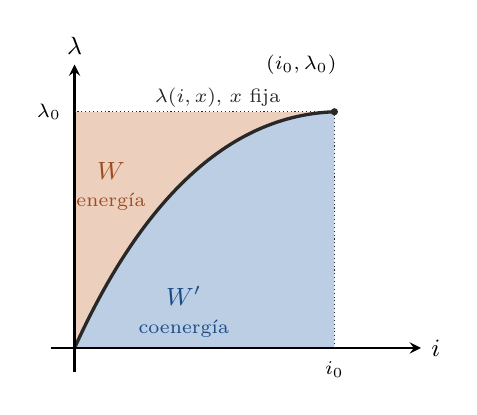
\begin{tikzpicture}[>=stealth, font=\small]
  \def\imax{4.4} \def\lmax{3.6}
  \def\izero{3.3} \def\lzero{3.0}
  % curva lambda(i) a x fija, forma de saturacion
  \pgfmathsetmacro{\curvepath}{0}
  % areas, dibujadas antes que los ejes para que estos queden encima
  \fill[tray!55, opacity=0.55]
    (0,0) .. controls (\izero*0.35,\lzero*0.85) and (\izero*0.75,\lzero*0.99) .. (\izero,\lzero)
    -- (\izero,0) -- cycle;
  \fill[ctl2!55, opacity=0.55]
    (0,0) .. controls (\izero*0.35,\lzero*0.85) and (\izero*0.75,\lzero*0.99) .. (\izero,\lzero)
    -- (0,\lzero) -- cycle;
  % curva encima de las areas
  \draw[very thick, refc] (0,0) .. controls (\izero*0.35,\lzero*0.85) and (\izero*0.75,\lzero*0.99) .. (\izero,\lzero);
  % ejes
  \draw[->, thick] (-0.3,0) -- (\imax,0) node[right] {$i$};
  \draw[->, thick] (0,-0.3) -- (0,\lmax) node[above] {$\lambda$};
  % guias punteadas al punto de operacion
  \draw[densely dotted, refc] (\izero,0) -- (\izero,\lzero) -- (0,\lzero);
  \fill[refc] (\izero,\lzero) circle (1.3pt);
  \node[anchor=south east, font=\scriptsize] at (\izero+0.15,\lzero+0.35) {$(i_0,\lambda_0)$};
  \node[anchor=north, font=\scriptsize] at (\izero,-0.05) {$i_0$};
  \node[anchor=east, font=\scriptsize] at (-0.05,\lzero) {$\lambda_0$};
  % etiquetas de las areas (apiladas, para que no se encimen)
  \node[tray!80!black, font=\small] at (\izero*0.42,\lzero*0.22) {$W'$};
  \node[tray!80!black, font=\scriptsize] at (\izero*0.42,\lzero*0.08) {coenergía};
  \node[ctl2!80!black, font=\small] at (\izero*0.14,\lzero*0.75) {$W$};
  \node[ctl2!80!black, font=\scriptsize] at (\izero*0.14,\lzero*0.62) {energía};
  % curva etiquetada, lejos del punto de operacion para no encimarse
  \node[refc, font=\scriptsize, anchor=south, yshift=4pt] at (\izero*0.55,\lzero*0.93) {$\lambda(i,x)$, $x$ fija};
\end{tikzpicture}

    \caption[Energía y coenergía magnética]{Energía $W$ y coenergía $W'$ como las dos áreas en que la curva $\lambda(i,x)$, a posición $x$ fija, divide el rectángulo del punto de operación $(i_0,\lambda_0)$. Cuando la corriente es la variable que se fija externamente, como ocurre en este trabajo, la fuerza mecánica se obtiene derivando la coenergía, $F=+\partial W'/\partial x$, no la energía.}
    \label{fig:energia_coenergia}
\end{figure}

Para un circuito magnético lineal, con inductancia $L(x)$ independiente de la corriente, la coenergía tiene la forma particularmente simple $W'(x,i)=\tfrac12 L(x)\,i^2$, y su derivada reproduce exactamente la fuerza de reluctancia~\eqref{eq:fld_reluctancia} de la subsección anterior, $f_{\text{rel}}=\tfrac12 i^2\,dL/dx$: ese resultado, obtenido ahí por un argumento distinto, es un caso particular de lo que aquí se presenta en general. La fuerza del fabricante~\eqref{eq:fld} crece con $u$ de forma lineal, no cuadrática, de modo que la coenergía que la reproduce no puede tener la forma $\tfrac12 L(x)i^2$ de un circuito puramente inductivo; esto no exige, por sí solo, que el circuito magnético sea no lineal, porque una fuerza lineal en la corriente también aparece en un circuito lineal con flujo de un imán permanente, $\lambda(x,i)=L_0 i+\lambda_{\text{pm}}(x)$, cuyo término de interacción $i\,\lambda_{\text{pm}}(x)$ es lineal en $i$. Lo que se construye aquí es ese término de interacción, sin derivar la energía electromagnética completa del dispositivo ni pronunciarse sobre la linealidad de su circuito. Lo que sí se conserva del caso lineal es el método: proponer una función $W'(x,u)$ cuya derivada respecto a $x$ sea la fuerza conocida,
\begin{equation}
W'(x,u) = \frac{u}{3b(a-x)^3} ,
\label{eq:coenergia}
\end{equation}
que cumple, por construcción, $\partial W'/\partial x = f_{\text{fld}}(u,x)$, la fuerza del fabricante~\eqref{eq:fld}. El voltaje $u$ se trata en~\eqref{eq:coenergia} como un parámetro externo y no como una variable dinámica propia: el circuito del embobinado es resistivo y su constante de tiempo eléctrica es mucho menor que la mecánica (subsección~\ref{sec:fuerza_primeros_principios}), de modo que $u$ fija de forma cuasiestática la corriente, y con ella la coenergía, sin que haga falta escribir una ecuación de movimiento aparte para el circuito eléctrico.

La figura~\ref{fig:coenergia_posicion} muestra la coenergía~\eqref{eq:coenergia} para tres voltajes representativos del intervalo de operación de este trabajo. Crece con el voltaje, como corresponde a una cantidad asociada al campo magnético, y crece con mucha más fuerza al acercarse a la bobina ($x\to a$) que al alejarse: esa asimetría es la que, al derivar respecto a $x$, produce una fuerza que aumenta como la cuarta potencia del inverso del entrehierro, y es la raíz última de la inestabilidad en lazo abierto que la sección~\ref{sec:linealizado} analiza.

\begin{figure}[ht]
    \centering
    % Coenergia magnetica W'(x,u) = u/(3 b (a-x)^3) contra la posicion, para tres
% voltajes representativos del intervalo de operacion de este trabajo.
% Valores: a=7.17184 cm, b=1.6163e-6 (tabla de parametros).
\definecolor{tray}{RGB}{31,94,166}
\definecolor{ctl2}{RGB}{196,96,40}
\definecolor{ver}{RGB}{46,133,64}
\begin{tikzpicture}
\begin{axis}[
    width=0.85\textwidth, height=6cm,
    grid=major, grid style={gray!25},
    tick label style={font=\small}, label style={font=\small}, legend style={font=\small},
    scaled ticks=false,
    xlabel={posición $x_1$ [\si{cm}]}, ylabel={coenergía $W'$ [\si{kg.cm^2/s^2}]},
    xmin=-4, xmax=-2, ymin=0, ymax=950,
    legend style={at={(0.02,0.98)}, anchor=north west}, legend cell align=left,
    domain=-4:-2, samples=60,
]
  \addplot[tray, thick] {1.5/(3*1.6163e-6*(7.17184-x)^3)};
  \addlegendentry{$u=1.5$~V}
  \addplot[ctl2, thick] {2.0/(3*1.6163e-6*(7.17184-x)^3)};
  \addlegendentry{$u=2.0$~V}
  \addplot[ver, thick] {2.5/(3*1.6163e-6*(7.17184-x)^3)};
  \addlegendentry{$u=2.5$~V}
\end{axis}
\end{tikzpicture}

    \caption[Coenergía magnética contra la posición]{Coenergía $W'(x,u)$ de~\eqref{eq:coenergia} contra la posición del imán, para tres voltajes del intervalo de operación. Crece con el voltaje y, para cualquier voltaje fijo, mucho más al acercarse a la bobina que al alejarse de ella.}
    \label{fig:coenergia_posicion}
\end{figure}

\paragraph{El lagrangiano y la ecuación de Euler-Lagrange.}
Con la energía cinética~\eqref{eq:cinetica_cap3}, la energía potencial gravitacional~\eqref{eq:potencial_grav} y la coenergía de acoplamiento~\eqref{eq:coenergia}, el lagrangiano del sistema, sin ningún término de fricción, es
\begin{equation}
L(x,\dot{x}) = \underbrace{\frac{1}{2}m\dot{x}^2}_{T} \;-\; \underbrace{mgx}_{V_{\text{grav}}} \;+\; \underbrace{W'(x,u)}_{\text{acoplamiento}} .
\label{eq:lagrangiano}
\end{equation}
Conviene detenerse en los signos de~\eqref{eq:lagrangiano}: la energía cinética entra con signo positivo y la potencial con signo negativo, como en cualquier lagrangiano $L=T-V$; la coenergía de acoplamiento entra también con signo positivo, no porque sea cinética, sino por la razón opuesta de signo entre energía y coenergía que explica la figura~\ref{fig:energia_coenergia}. Omitir ese signo, por analogía con una energía potencial ordinaria, invertiría el sentido de la fuerza magnética en la ecuación de movimiento. Sustituyendo~\eqref{eq:lagrangiano} en la ecuación de Euler-Lagrange~\eqref{eq:euler_lagrange} se obtiene
\begin{equation}
\frac{\partial L}{\partial \dot x} = m\dot x, \qquad
\frac{d}{dt}\left(\frac{\partial L}{\partial \dot x}\right) = m\ddot x, \qquad
\frac{\partial L}{\partial x} = -mg + \frac{\partial W'}{\partial x} = f_{\text{fld}}(u,x) - mg ,
\label{eq:el_pasos}
\end{equation}
de modo que~\eqref{eq:euler_lagrange} da $m\ddot{x} = f_{\text{fld}}(u,x) - mg$, idéntica a la ecuación de movimiento~\eqref{eq:mec} sin el término de fricción $f_{\text{fr}}$.

\paragraph{Verificación cruzada: las ecuaciones de Hamilton.}
Como verificación independiente de~\eqref{eq:el_pasos}, se repitió el cálculo con el formalismo hamiltoniano, que parte del mismo lagrangiano pero reorganiza la dinámica en términos de la posición $x$ y el momento canónico $p$, en vez de la posición y la velocidad. El momento canónico es
\begin{equation}
p = \frac{\partial L}{\partial \dot{x}} = m\dot{x} ,
\label{eq:momento_canonico}
\end{equation}
y la transformada de Legendre del lagrangiano~\eqref{eq:lagrangiano}, $H=p\dot x - L$, expresada en términos de $p$ en vez de $\dot x$, da el hamiltoniano
\begin{equation}
H(x,p) = \frac{p^2}{2m} - W'(x,u) + mgx .
\label{eq:hamiltoniano}
\end{equation}
Las ecuaciones de Hamilton, $\dot{x}=\partial H/\partial p$ y $\dot{p}=-\partial H/\partial x$, dan
\begin{equation}
\dot{x} = \frac{p}{m} , \qquad \dot{p} = f_{\text{fld}}(u,x) - mg .
\label{eq:hamilton_ec}
\end{equation}
Derivando la primera ecuación de~\eqref{eq:hamilton_ec} respecto al tiempo y sustituyendo la segunda se recupera $m\ddot x = f_{\text{fld}}(u,x)-mg$, la misma ecuación que con Lagrange, obtenida esta vez a partir del momento canónico en lugar de la velocidad. Las dos verificaciones, simbólicas e independientes entre sí, se hicieron mediante cálculo simbólico. Conviene precisar qué prueba este acuerdo y qué no: Lagrange y Hamilton son dos formulaciones equivalentes del mismo lagrangiano~\eqref{eq:lagrangiano}, así que su coincidencia verifica que el álgebra se hizo bien, no que la coenergía~\eqref{eq:coenergia} sea la energía electromagnética físicamente correcta del dispositivo. La construcción parte de la fuerza del fabricante ya adoptada e integra para obtener $W'$; volver a derivarla reproduce, por diseño, la misma fuerza. Esta subsección es, por tanto, una verificación de consistencia interna del modelo mecánico sin fricción, complementaria del límite dipolo-dipolo de la subsección anterior, y no una validación física independiente de la ley de fuerza del fabricante.

\section{Fricción con atascamiento-deslizamiento}\label{sec:friccion_modelo}

La sección~\ref{sec:fund_friccion} describió las componentes de la fricción y el método de Karnopp en general. Esta sección precisa cómo se aplican al imán.

En este trabajo se emplea un modelo de fricción compuesto. Con velocidad nula, el imán está en régimen de fricción estática; cuando la fuerza externa lo pone en movimiento, la fricción disminuye de golpe y pasa al régimen de fricción dinámica. La fuerza de fricción es
\begin{equation}
f_{\text{fr}} =
\begin{cases}
m\,c_1\,v,
& v \neq 0, \\[6pt]
\min\!\left(|F_e|,\,F_s\right)\,\operatorname{sign}(F_e),
& v = 0 .
\end{cases}
\label{eq:friccion}
\end{equation}
En el régimen de deslizamiento, la fricción~\eqref{eq:friccion} es viscosa y proporcional a la velocidad $v$ del imán, con el coeficiente $c_1$ de fricción viscosa por unidad de masa. En reposo, la fricción equilibra la fuerza externa $F_e(t)$ que actúa sobre el imán, es decir, la suma de la fuerza electromagnética y el peso, hasta un valor máximo $F_s$, la fricción estática máxima.

La discontinuidad de la fricción en la velocidad cero es una dificultad más numérica que física, y existe una amplia variedad de estrategias para implementarla, conocidas como modelos dinámicos de fricción~\cite{haessig}. Aquí se emplea el método de Karnopp~\cite{karnopp}, por su fácil implementación. Con él, el imán se considera detenido mientras su velocidad cumple $|v| \le DV$, con la banda de velocidad nula $DV$ de la tabla~\ref{tab:parametros}, y la ecuación~\eqref{eq:friccion} decide si la fuerza externa lo mantiene atascado o lo libera.

\section{Zona muerta centrada en el voltaje de equilibrio}\label{sec:zm_modelo}

Pérez-Gómez~\cite{perez} sostiene que la zona muerta dura describe con mayor precisión el fenómeno observado en motores eléctricos, en los que esta no linealidad se centra en $u_e(t) = 0$, el único voltaje de equilibrio de los sistemas de control de posición angular.

En los sistemas de levitación magnética, en cambio, cada posición tiene su propio voltaje de equilibrio $u_e$~\eqref{eq:ue}, y la zona muerta se centra en él,
\begin{equation}
v(t) = D\big(u(t)\big) =
\begin{cases}
m_r \big(u(t) - u_e - b_r\big) - h_r, & u(t) - u_e \ge b_r, \\[6pt]
0, & b_l < u(t) - u_e < b_r, \\[6pt]
m_l \big(u(t) - u_e - b_l\big) - h_l, & u(t) - u_e \le b_l.
\end{cases}
\label{eq:zm}
\end{equation}
La zona muerta~\eqref{eq:zm} transforma el voltaje comandado $u$ en la salida $v$ del actuador. En esta ecuación, y en la figura~\ref{fig:zm} y el lazo de la figura~\ref{lazo_de_control_con_zm}, $v$ denota la salida de la zona muerta y no la velocidad del imán, que en el resto del capítulo se designa con el mismo símbolo. Mientras la desviación $u-u_e$ permanece entre los umbrales $b_l$ y $b_r$, la salida es nula. Fuera de esa banda, la salida crece con las pendientes $m_r$ y $m_l$ y se desplaza por los saltos $h_r$ y $h_l$. Estos seis parámetros son desconocidos, pero sus signos se conocen: $m_r > 0$, $m_l > 0$, $b_r > 0$, $b_l < 0$, $h_r < 0$ y $h_l > 0$.


\begin{figure}[ht]
    \centering
    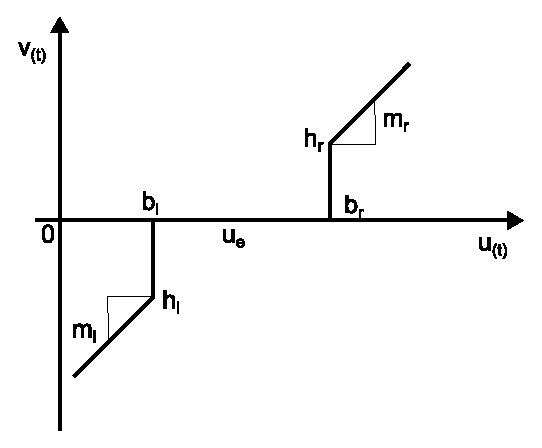
\includegraphics[width=0.45\textwidth]{images/chapter_1/zm_levitador.eps}
    \caption[Zona muerta centrada en el voltaje de equilibrio]{Zona muerta $v=D(u)$ centrada en el voltaje de equilibrio $u_e$, con pendientes $m_l$, $m_r$, umbrales $b_l$, $b_r$ y saltos $h_l$, $h_r$.}
    \label{fig:zm}
\end{figure}

La figura~\ref{fig:zm} muestra la forma de $D(u)$: mientras el voltaje comandado se mantenga dentro de la banda $(u_e+b_l,\,u_e+b_r)$, la salida $v$ del actuador es nula.

Como los parámetros de $D(u)$ no se conocen para el ECP-730, en las simulaciones se emplea una implementación simplificada con la misma asimetría de signos. Mientras el imán está en movimiento, el actuador no responde a cambios del voltaje comandado comprendidos entre $-0{,}02$ y $+0{,}025$~V respecto al último voltaje aplicado, que se mantiene; los cambios mayores se transmiten sin modificación. Cuando el imán está atascado, el voltaje comandado se aplica directamente. Esta implementación no es equivalente a $D(u)$. Tiene memoria, porque compara con el último voltaje aplicado en lugar de con $u_e$, y se desactiva mientras el imán está atascado. Los resultados de simulación valen, por tanto, para esta retención de voltaje y no para una zona muerta estática identificada del ECP-730. En una simulación adicional sin zona muerta, el ciclo límite del PII persiste con una amplitud un 8\,\% menor, de modo que la oscilación no necesita esta retención para aparecer. La identificación de los parámetros de $D(u)$ se propone como trabajo futuro.

La figura~\ref{lazo_de_control_con_zm} muestra el lazo de control completo, con la zona muerta entre el controlador y la planta.

\begin{figure}[ht]
    \centering
       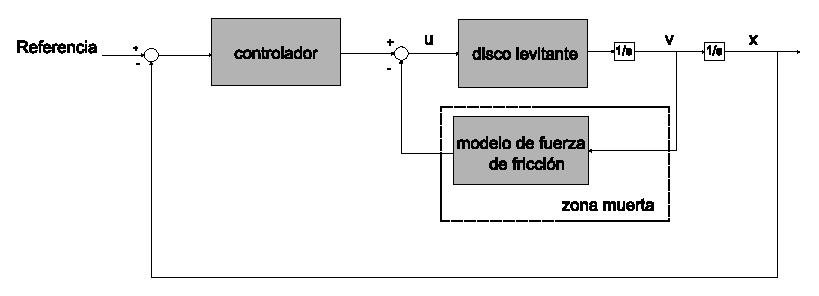
\includegraphics[width=0.6\textwidth]{images/chapter_1/lazo_de_control_con_zm.eps}
    \caption{Lazo de control con zona muerta}
    \label{lazo_de_control_con_zm}
\end{figure}

\section{Parámetros del modelo}\label{sec:parametros}

Los parámetros del modelo no lineal ($a$, $b$, $c_1$, $m$, $g$) fueron identificados experimentalmente por Hernández Alcántara~\cite{diana_tesis} para el dispositivo ECP-730 en configuración repulsiva (estable en lazo abierto), mediante ensayos de estado estacionario y respuesta dinámica en lazo abierto. En el presente trabajo se adoptan esos mismos parámetros y se aplican a la configuración atractiva (inestable en lazo abierto), en la que la bobina superior atrae al imán. La estructura funcional del modelo es idéntica en ambas configuraciones; en la atractiva, la fuerza magnética crece al disminuir la brecha entre el imán y la bobina, lo que hace que los puntos de equilibrio sean inestables.

La tabla~\ref{tab:parametros} reúne estos valores junto con los parámetros del modelo de fricción, el intervalo de la señal de control y la banda de la zona muerta simulada. Las fuerzas se expresan en $\text{kg}\cdot\text{cm}/\text{s}^2$, unidades en las que el peso del imán es $mg = 138{,}3$. En la tesis de Hernández Alcántara~\cite{diana_tesis}, $c_1$ se reporta en $\text{kg}^{-1}$; dado que multiplica a la velocidad en la ecuación de aceleración, sus unidades consistentes son $\text{s}^{-1}$. Por la misma razón, el valor de $b$ corresponde a fuerzas en $\text{kg}\cdot\text{cm}/\text{s}^2$, es decir, a voltios por $(\text{kg}\cdot\text{cm}/\text{s}^2)\cdot\text{cm}^4$. Ese antecedente lo reporta en $\text{V}/(\text{N}\cdot\text{cm}^4)$, y con esa unidad el valor equivalente sería $1{,}6163\times10^{-4}$, cien veces mayor. Con el valor y la unidad de la tabla~\ref{tab:parametros}, el modelo reproduce los voltajes de equilibrio que se usan en todo el trabajo.


\begin{table}[ht]
\centering
\caption{Parámetros del modelo}
\label{tab:parametros}
\begin{tabular}{|c|c|l|}
\hline
$a$ & $7{,}17184\;[\text{cm}]$ & parámetro de la fuerza electromagnética \\ \hline
$b$ & $1{,}6163 \times 10^{-6}\;[\text{V}\cdot\text{s}^2/(\text{kg}\cdot\text{cm}^5)]$ & parámetro de la fuerza electromagnética \\ \hline
$c_1$ & $8{,}563\;[\text{s}^{-1}]$ & fricción viscosa por unidad de masa \\ \hline
$m$ & $0{,}141\;[\text{kg}]$ & masa del imán \\ \hline
$g$ & $981\;[\text{cm}/\text{s}^2]$ & aceleración de la gravedad \\ \hline
$F_s$ & $20\;[\text{kg}\cdot\text{cm}/\text{s}^2]$ ($0{,}2$~N) & fricción estática máxima (Karnopp) \\ \hline
$DV$ & $0{,}02\;[\text{cm}/\text{s}]$ & banda de velocidad nula (Karnopp) \\ \hline
$u$ & $[0;\ 3{,}5]\;[\text{V}]$ & intervalo de la señal de control \\ \hline
$[b_l,\,b_r]$ & $[-0{,}02;\ +0{,}025]\;[\text{V}]$ & banda de la zona muerta simulada \\ \hline
\end{tabular}
\end{table}

\section{Modelo linealizado}\label{sec:linealizado}

Para diseñar el controlador se linealiza el modelo alrededor de una posición de equilibrio $x_1^{\ast}$, con el procedimiento general de la sección~\ref{sec:fund_linealizacion}. El modelo linealizado en espacio de estados para la configuración inestable es

\begin{equation}
\begin{aligned}
\dot{x}
&=
\begin{bmatrix}
0 & 1 \\[6pt]
\dfrac{4g}{(a-x_1^{\ast})} & -c_1
\end{bmatrix}x
+
\begin{bmatrix}
0 \\[6pt]
\dfrac{1}{mb\,(a-x_1^{\ast})^4}
\end{bmatrix}u,
\\[10pt]
y &= \begin{bmatrix} 1 & 0 \end{bmatrix} x .
\end{aligned}
\label{eq:lineal}
\end{equation}
En el modelo linealizado~\eqref{eq:lineal}, el vector de estado $x$ reúne la posición $x_1$ y la velocidad $x_2$ del imán, y la salida $y$ es la posición. El coeficiente $c_1$ de fricción viscosa por unidad de masa aparece en la matriz de estado como un amortiguamiento.

Su ecuación característica es
\begin{equation}
\lambda^2 + c_1\lambda - \dfrac{4g}{(a-x_1^{\ast})} = 0 .
\label{eq:caracteristica}
\end{equation}
Como $a - x_1^{\ast} > 0$ para toda posición alcanzable, el término independiente de la ecuación característica~\eqref{eq:caracteristica} es negativo y la ecuación tiene siempre una raíz real positiva: todos los puntos de equilibrio de la configuración atractiva son inestables. En $x_1^{\ast}=-4$~cm las raíces son $\lambda_1 = -23{,}5057$ y $\lambda_2 = 14{,}9427$.

Las matrices de controlabilidad y de observabilidad del modelo linealizado son
\begin{equation}
\mathcal{C}
=
\begin{bmatrix}
0 & \beta\\[6pt]
\beta & -c_1 \beta
\end{bmatrix} ,
\qquad
\mathcal{O}
=
\begin{bmatrix}
1 & 0\\[6pt]
0 & 1
\end{bmatrix} .
\label{eq:ctrb_obsv}
\end{equation}
La constante $\beta = 1/[m\,b\,(a-x_1^{\ast})^4]$ es la ganancia con la que el voltaje entra en la aceleración del imán. Las dos matrices~\eqref{eq:ctrb_obsv} tienen rango completo, de modo que el sistema es controlable y observable: con la entrada de la planta se puede llevar el estado a cualquier punto del espacio de estados, y a partir de la salida se puede determinar en qué punto se encuentra.

% Generado a partir de calculus/Final_Bien/evidencia_P8.m (simulador corregido).
\section{Comportamiento en lazo abierto}\label{sec:lazo_abierto}

Para caracterizar la inestabilidad de la configuración atractiva, se simuló el modelo no lineal sin fricción estática ni zona muerta, aplicando el voltaje de equilibrio $u=u_e(x_1^*)$ y desplazando la posición inicial $0{,}01$~cm respecto al equilibrio, en $x_1^*=-4$, $-3$ y $-2$~cm. La figura~\ref{fig:p8_lazo_abierto} muestra que la desviación crece exponencialmente y alcanza 1~cm en $0{,}33$, $0{,}32$ y $0{,}30$~s, respectivamente; el modelo linealizado reproduce el crecimiento con un tiempo de duplicación $\ln 2/\lambda_2$ de $46$, $44$ y $41$~ms. Cuanto más cerca de la bobina se encuentra el equilibrio, más rápido es el polo inestable.

\begin{figure}[ht]
    \centering
    % Estilo común de las figuras de evidencia P8 (pgfplots).
\pgfplotsset{
  pocho/.style={
    width=0.92\textwidth, height=5.2cm,
    grid=major, grid style={gray!25},
    tick label style={font=\small}, label style={font=\small}, legend style={font=\small},
    scaled ticks=false,
    y tick label style={/pgf/number format/fixed},
    table/col sep=comma, unbounded coords=jump,
    every axis plot/.append style={line join=round},
  },
}
\definecolor{tray}{RGB}{31,94,166}
\definecolor{refc}{RGB}{40,40,40}
\definecolor{ctl2}{RGB}{196,96,40}
\definecolor{ver}{RGB}{46,133,64}

\begin{tikzpicture}
\begin{semilogyaxis}[pocho, height=6cm, xmin=0, xmax=0.36, ymin=0.01, ymax=1,
    xlabel={tiempo [\si{s}]}, ylabel={$|x_1(t)-x_1^*|$ [\si{cm}]},
    x tick label style={/pgf/number format/fixed},
    legend style={at={(0.02,0.98)}, anchor=north west}, legend cell align=left]
  \addplot[tray, line width=1pt]  table[x=t, y=nl_m4] {images/p8_results/tikz/lazo_abierto.csv}; \addlegendentry{$x_1^*=-4$ cm}
  \addplot[ctl2, line width=1pt]  table[x=t, y=nl_m3] {images/p8_results/tikz/lazo_abierto.csv}; \addlegendentry{$x_1^*=-3$ cm}
  \addplot[ver, line width=1pt]   table[x=t, y=nl_m2] {images/p8_results/tikz/lazo_abierto.csv}; \addlegendentry{$x_1^*=-2$ cm}
  \addplot[tray, densely dashed]  table[x=t, y=lin_m4] {images/p8_results/tikz/lazo_abierto.csv}; \addlegendentry{modelo lineal}
  \addplot[ctl2, densely dashed, forget plot] table[x=t, y=lin_m3] {images/p8_results/tikz/lazo_abierto.csv};
  \addplot[ver, densely dashed, forget plot]  table[x=t, y=lin_m2] {images/p8_results/tikz/lazo_abierto.csv};
\end{semilogyaxis}
\end{tikzpicture}

    \caption[Lazo abierto en los puntos de equilibrio]{Desviación respecto al equilibrio en lazo abierto, con $u=u_e$ y una perturbación inicial de $0{,}01$~cm. Líneas continuas: modelo no lineal; discontinuas: modelo linealizado.}
    \label{fig:p8_lazo_abierto}
\end{figure}

El retrato de fase alrededor de $x_1^*=-4$~cm (figura~\ref{fig:p8_retrato}) confirma que el equilibrio es un punto silla: las trayectorias se alejan a lo largo de la variedad inestable, salvo las que parten exactamente sobre la variedad estable.


\begin{figure}[ht]
    \centering
    % Estilo común de las figuras de evidencia P8 (pgfplots).
\pgfplotsset{
  pocho/.style={
    width=0.92\textwidth, height=5.2cm,
    grid=major, grid style={gray!25},
    tick label style={font=\small}, label style={font=\small}, legend style={font=\small},
    scaled ticks=false,
    y tick label style={/pgf/number format/fixed},
    table/col sep=comma, unbounded coords=jump,
    every axis plot/.append style={line join=round},
  },
}
\definecolor{tray}{RGB}{31,94,166}
\definecolor{refc}{RGB}{40,40,40}
\definecolor{ctl2}{RGB}{196,96,40}
\definecolor{ver}{RGB}{46,133,64}

\begin{tikzpicture}
\begin{axis}[pocho, width=0.8\textwidth, height=7.5cm, xmin=-4.5, xmax=-3.5, ymin=-10, ymax=10,
    xlabel={posición $x_1$ [\si{cm}]}, ylabel={velocidad $x_2$ [\si{cm/s}]},
    legend style={at={(0.98,0.02)}, anchor=south east, fill=white}, legend cell align=left]
  \addplot[gray!60, quiver={u=\thisrow{dx}, v=\thisrow{dv}, every arrow/.append style={-stealth}}, forget plot]
    table[x=x, y=v] {images/p8_results/tikz/campo.csv};
  \addplot[tray, line width=0.9pt] table[x=x, y=v] {images/p8_results/tikz/trayectorias.csv}; \addlegendentry{trayectorias}
  \addplot[ctl2, line width=1.4pt] table[x=x, y=v] {images/p8_results/tikz/variedad_inestable.csv}; \addlegendentry{variedad inestable}
  \addplot[ver, line width=3pt, opacity=0.6] coordinates {(-4.4448,0) (-3.6291,0)}; \addlegendentry{banda de atascamiento ($u=u_e$)}
  \addplot[only marks, mark=*, mark size=2pt, refc] coordinates {(-4,0)}; \addlegendentry{equilibrio $x_1^*=-4$ cm}
\end{axis}
\end{tikzpicture}

    \caption[Retrato de fase en lazo abierto]{Retrato de fase del modelo no lineal sin fricción estática alrededor de $x_1^*=-4$~cm, con $u=u_e$. La banda verde indica las posiciones en las que, con el imán en reposo, la fricción estática lo mantiene atascado.}
    \label{fig:p8_retrato}
\end{figure}

Al incorporar la fricción estática de Karnopp cambia la situación en reposo: si el imán está detenido y $u=u_e$, la fuerza neta $u/[b(a-x)^4]-mg$ no supera $F_s$ mientras la posición se encuentre entre $-4{,}44$ y $-3{,}63$~cm, de modo que el imán permanece atascado en cualquier punto de esa banda. Para $x_1^*=-3$ y $-2$~cm las bandas correspondientes son $[-3{,}41;\,-2{,}66]$ y $[-2{,}37;\,-1{,}70]$~cm. La fricción estática enmascara así la inestabilidad del equilibrio mientras el imán no se mueva.

\FloatBarrier

\section{Análisis estático del actuador}\label{sec:actuador_estatico}

El voltaje que puede aplicar el actuador está acotado a $u\in[0;\,3{,}5]$~V, y esa cota determina en qué posiciones puede operar el sistema. Para sostener el imán en $x_1$ se necesita el voltaje de equilibrio~\eqref{eq:ue}, que crece rápidamente al alejarse de la bobina: $1{,}58$~V en $-2$~cm, $2{,}39$~V en $-3$~cm, $3{,}48$~V en $-4$~cm y $4{,}91$~V en $-5$~cm. Para mover el imán hay que vencer además la fricción estática, lo que exige llegar a $u_e(1\pm F_s/mg)$, es decir, a un $14{,}5$\,\% por encima o por debajo del equilibrio. La sección~\ref{sec:analisis_ciclo} retoma esta banda para explicar el ciclo límite.

En $x_1=-4$~cm, el punto en que se linealizó el modelo para el diseño, el imán puede sostenerse con $3{,}48$~V, pero no subir: para despegarlo hacia la bobina se requieren unos $3{,}99$~V, por encima de la cota de $3{,}5$~V. Sí puede despegarse hacia abajo si el voltaje baja de unos $2{,}98$~V, pero entonces se aleja de la bobina, el voltaje de equilibrio crece todavía más y el actuador ya no puede recuperarlo. Desde $-4$~cm el imán no tiene, por tanto, ningún movimiento regulable, aunque sí puede caer. El barrido de escalones del capítulo~\ref{chap:desempeno} determina qué posiciones y qué cambios de referencia son alcanzables con $u\le3{,}5$~V, y de él se obtiene el intervalo de pruebas.

El modelo queda así completo: una planta inestable en lazo abierto, con fricción estática que puede mantener al imán detenido y un actuador acotado, con zona muerta, que limita dónde se puede actuar. Sobre el modelo linealizado se diseña, en el capítulo siguiente, el controlador.
